\section{Tree on the vertices}

\begin{frame}{Tree on the vertices}

\probBook + tree:

\begin{overprint}
\onslide<1>
\begin{figure}\centering
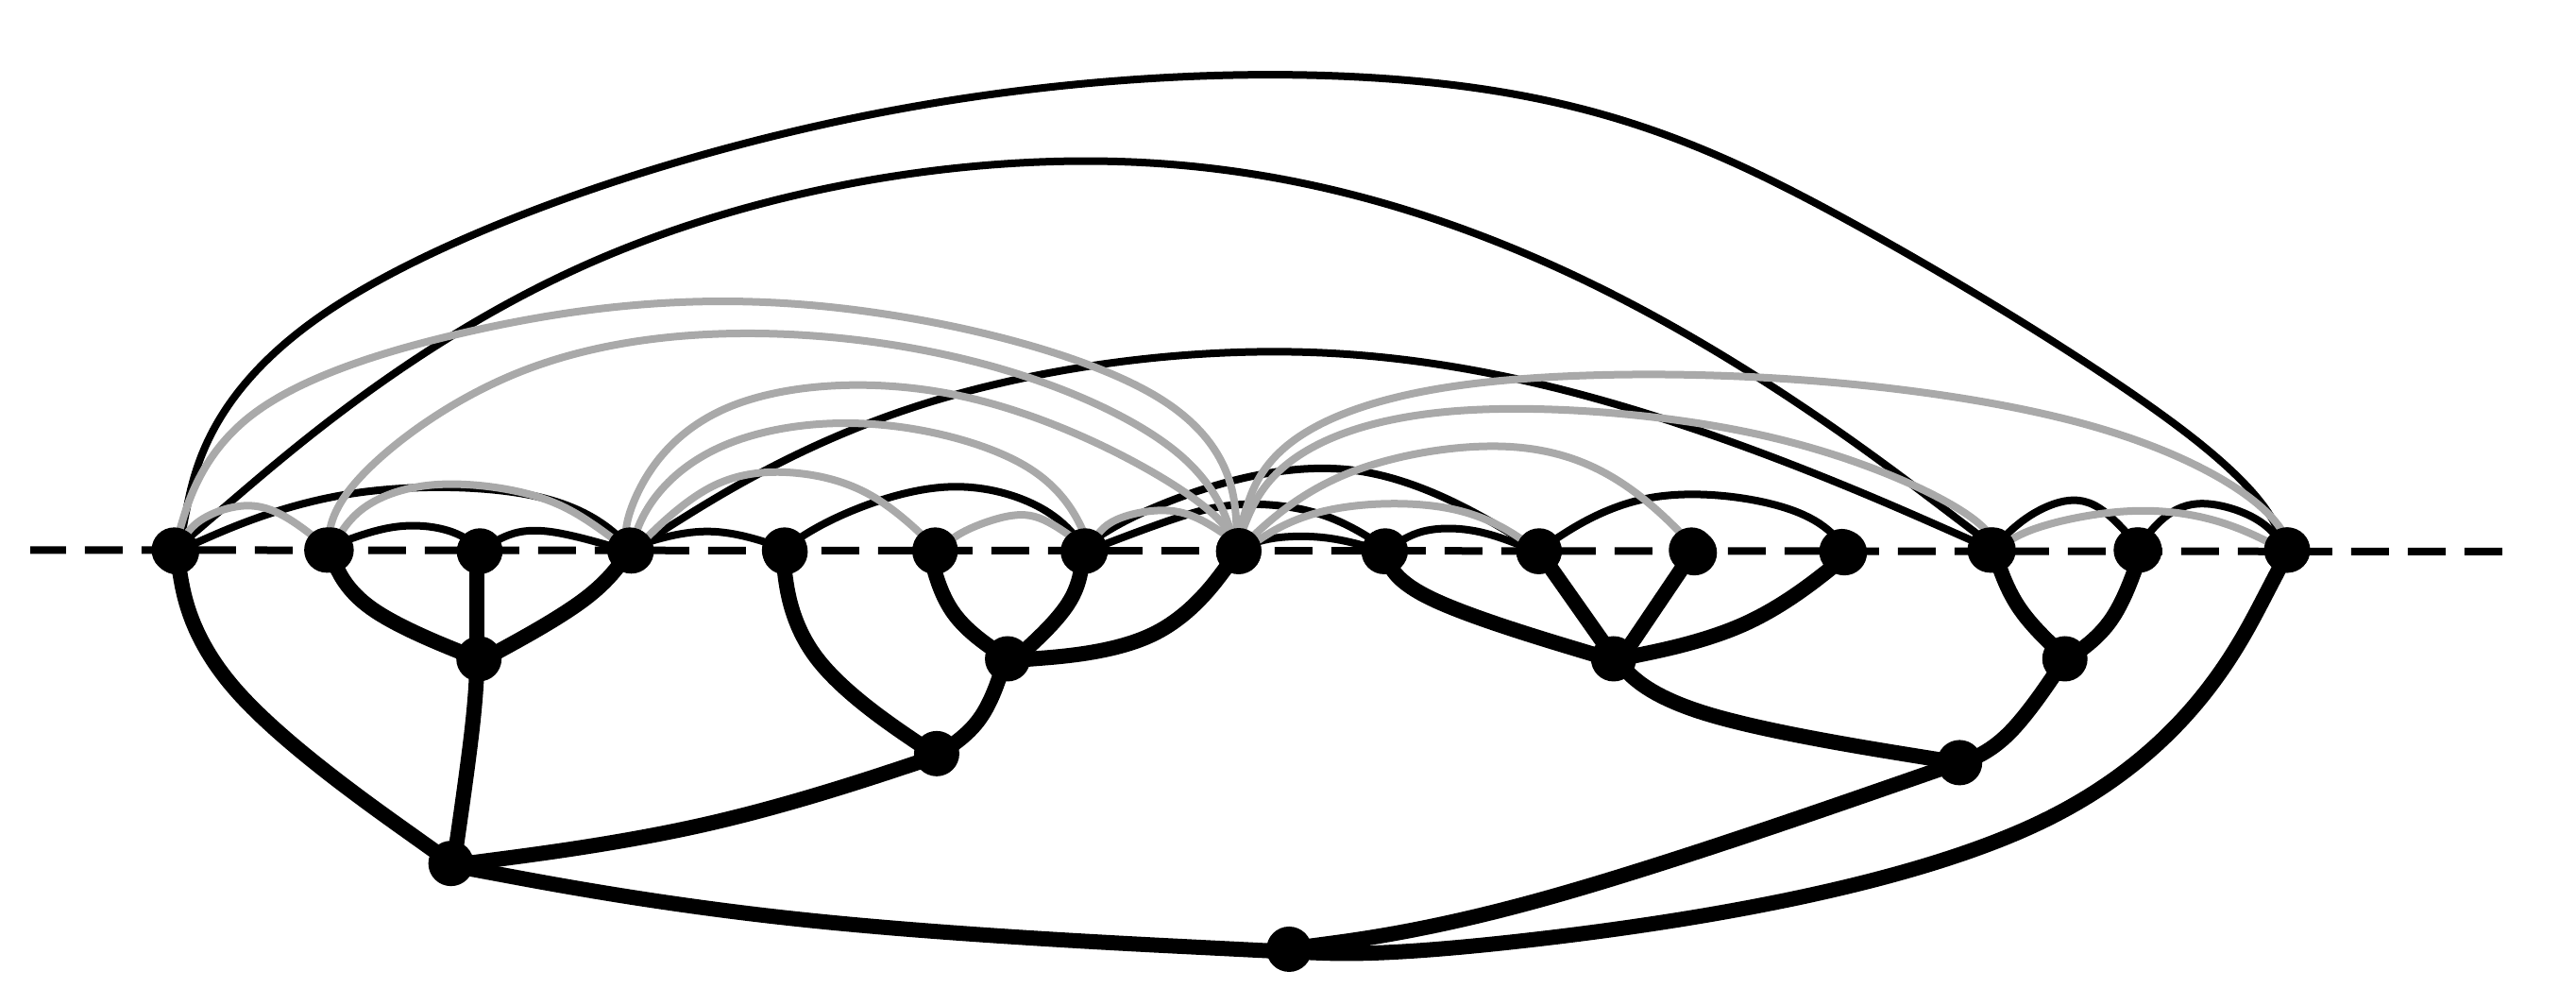
\includegraphics[width=0.8\textwidth]{sefe2}
\end{figure}

Drawing the tree = Restricting permutations by a \PT-tree

\onslide<2>
\vspace{-1em}
\newProb{\probPTree}{\probBook instance $I$ and a \PT-tree~$T$ with leaves~$V$.}{Is there a total order $<\,\in \pi(T)$ solving $I$?}

More structure (same for binary trees):
\newProb{\probQTree}{\probBook instance $I$ and a \Q-tree~$T$ with leaves~$V$.}{Is there a total order $<\,\in \pi(T)$ solving $I$?}
\end{overprint}
\end{frame}

\begin{frame}{Example}

\begin{overprint}

\onslide<1>
\begin{figure}
\centering
\scalebox{1.0}{%
\begin{tikzpicture}
% ab || cd
\begin{scope}
\node (a) {a};
\node[right of=a] (b) {b};
\node[right of=b] (c) {c};
\node[right of=c] (d) {d};

\node[rectangle, draw] (c1) at ($ 0.5*($(a) + (b)$) + (0, -2em) $) {};
\node[rectangle, draw] (c2) at ($ 0.5*($(c) + (d)$) + (0, -2em) $) {};

\draw (c1) edge (a.south);
\draw (c1) edge (b.south);
\draw (c2) edge (c.south);
\draw (c2) edge (d.south);
\draw (c2) edge[bend left] (c1);
\end{scope}

\drawedges[bend left,edge1]{a/b,c/d}
\drawedges[bend left,edge1]{b/c,a/d}
\end{tikzpicture}}
\end{figure}

\begin{itemize}
  \item What happens to the forbidden suborder constraint?
  \item[$\Rightarrow$] 2-CNF formula (Boolean equations) on orientation of \Q-nodes
\end{itemize}

\onslide<2>
\begin{figure}
\centering
\scalebox{1.0}{%
\begin{tikzpicture}
% ab || cd
\begin{scope}
\node (a) {a};
\node[right of=a] (b) {b};
\node[right of=b] (c) {c};
\node[right of=c] (d) {d};

\node[rectangle, draw] (c1) at ($ 0.5*($(a) + (b)$) + (0, -2em) $) {};
\node[rectangle, draw] (c2) at ($ 0.5*($(c) + (d)$) + (0, -2em) $) {};

\draw (c1) edge (a.south);
\draw (c1) edge (b.south);
\draw (c2) edge (c.south);
\draw (c2) edge (d.south);
\draw (c2) edge[bend left] (c1);
\end{scope}

\drawedges[bend left,white]{b/c,a/d}
\drawedges[bend left,edge1]{a/b,c/d}
\end{tikzpicture}}
\end{figure}

\begin{itemize}
\item $\{a, b\}$, $\{c, d\}$: \bool{true}
\end{itemize}
\onslide<3>

\begin{figure}
\centering
\scalebox{0.8}{%
\begin{tikzpicture}
% ab || cd
\begin{scope}
\node (a) {a};
\node[right of=a] (b) {b};
\node[right of=b] (c) {c};
\node[right of=c] (d) {d};

\node[rectangle, draw] (c1) at ($ 0.5*($(a) + (b)$) + (0, -2em) $) {};
\node[rectangle, draw] (c2) at ($ 0.5*($(c) + (d)$) + (0, -2em) $) {};
\node at ($ (c1) + (-.3,0)$) {r};
\node at ($ (c2) + (+.3,0)$) {s};

\draw (c1) edge (a.south);
\draw (c1) edge (b.south);
\draw (c2) edge (c.south);
\draw (c2) edge (d.south);
\draw (c2) edge[bend left] (c1);
\drawedges[bend left,edge1]{b/c,a/d}
\end{scope}

\begin{scope}[xshift=12em]
\node (a) {a};
\node[right of=a] (b) {b};
\node[right of=b] (c) {d};
\node[right of=c] (d) {c};

\node[rectangle, draw] (c1) at ($ 0.5*($(a) + (b)$) + (0, -2em) $) {};
\node[rectangle, draw] (c2) at ($ 0.5*($(c) + (d)$) + (0, -2em) $) {};

\draw (c1) edge (a.south);
\draw (c1) edge (b.south);
\draw (c2) edge (c.south);
\draw (c2) edge (d.south);
\draw (c2) edge[bend left] (c1);
\drawedges[bend left,edge1]{b/d,a/c}
\end{scope}

\begin{scope}[yshift=-6em]
\node (a) {b};
\node[right of=a] (b) {a};
\node[right of=b] (c) {c};
\node[right of=c] (d) {d};

\node[rectangle, draw] (c1) at ($ 0.5*($(a) + (b)$) + (0, -2em) $) {};
\node[rectangle, draw] (c2) at ($ 0.5*($(c) + (d)$) + (0, -2em) $) {};

\draw (c1) edge (a.south);
\draw (c1) edge (b.south);
\draw (c2) edge (c.south);
\draw (c2) edge (d.south);
\draw (c2) edge[bend left] (c1);
\drawedges[bend left,edge1]{a/c,b/d}
\end{scope}

\begin{scope}[yshift=-6em,xshift=12em]
\node (a) {b};
\node[right of=a] (b) {a};
\node[right of=b] (c) {d};
\node[right of=c] (d) {c};

\node[rectangle, draw] (c1) at ($ 0.5*($(a) + (b)$) + (0, -2em) $) {};
\node[rectangle, draw] (c2) at ($ 0.5*($(c) + (d)$) + (0, -2em) $) {};

\draw (c1) edge (a.south);
\draw (c1) edge (b.south);
\draw (c2) edge (c.south);
\draw (c2) edge (d.south);
\draw (c2) edge[bend left] (c1);
\drawedges[bend left,edge1]{b/c,a/d}
\end{scope}

\end{tikzpicture}}
\end{figure}

\begin{itemize}
\item $\{a, d\}$, $\{b, c\}$: $a < b \Leftrightarrow c < d$\\
\item Fix reference orientation of inner nodes~$r$
\item Boolean variable~$o_r$ for being in reference orientation  
\item[$\Rightarrow$] $o_r \Leftrightarrow o_s$
\end{itemize}
\end{overprint}
\end{frame}

%\begin{frame}{Quadratic-time decision}
%%Idea:
%\begin{itemize}
%\item Map to \probTwoSat instance
%\item Fix reference orientation of inner nodes~$r$ of~$T$
%\item Let Boolean variable $o_r$ express~$r$ being in reference orientation
%\item Constraint for two edges yields 2-\CNF formula in constant time
%\end{itemize}
%\end{frame}

%\begin{frame}{Conventions}
%\begin{itemize}
%  \item Let $(V, E_1, \dotsc, E_k)$ be the \probBook instance we consider and $T$~be the \Q-tree on the leaves~$V$ that the vertex order should come from
%  \item For all~$M \subseteq V$ let $r(M)$ be the lowest common ancestor of the vertices~$M$ in~$T$
%  \item Fix a reference orientation for all inner nodes~$r$ of~$T$
%  \item Let the Boolean variable~$o_r$ express~$r$ being in reference orientation 
%\end{itemize}
%\end{frame}

%%%%%%%%%%%%%%%%%%%%%%%%% Book constraints
\begin{frame}{Book constraints to 2-\CNF formula}

\begin{theorem}
\probQTree is solvable in $\OO(kn^2)$ time.
\end{theorem}

\vspace{-.5em}
{
\begin{tabular}{m{0.2\textwidth}m{0.8\textwidth}}


%%% ROW 1
\begin{figure}
\centering
\resizebox{0.2\textwidth}{!}{%
\begin{tikzpicture}
% ab || cd
\begin{scope}
\node (a) {a};
\node[right of=a] (b) {b};
\node[right of=b] (c) {c};
\node[right of=c] (d) {d};

\node[rectangle, draw] (c1) at ($ 0.5*($(a) + (b)$) + (0, -2em) $) {};
\node[rectangle, draw] (c2) at ($ 0.5*($(c) + (d)$) + (0, -2em) $) {};

\draw (c1) edge (a.south);
\draw (c1) edge (b.south);
\draw (c2) edge (c.south);
\draw (c2) edge (d.south);
\draw (c2) edge[bend left] (c1);
\end{scope}
\drawedges[bend left,edge1]{a/b,c/d}
\end{tikzpicture}}
\end{figure} &
\bool{true}\\[-2em]

%%% ROW 2
\begin{figure}
\centering

\resizebox{0.2\textwidth}{!}{%
\begin{tikzpicture}

% ac || bd
\begin{scope}[xshift=5cm]
\node (a) {a};
\node[right of=a] (b) {c};
\node[right of=b] (c) {b};
\node[right of=c] (d) {d};

\node[rectangle, draw] (c1) at ($ 0.5*($(a) + (b)$) + (0, -2em) $) {};
\node[rectangle, draw] (c2) at ($ 0.5*($(c) + (d)$) + (0, -2em) $) {};

\draw (c1) edge (a.south);
\draw (c1) edge (b.south);
\draw (c2) edge (c.south);
\draw (c2) edge (d.south);
\draw (c2) edge[bend left] (c1);
\drawedges[bend left,edge1]{a/c,b/d}
\end{scope}

\end{tikzpicture}}
\end{figure}
 
 & \bool{o_{r(a, c)} \Leftrightarrow o_{r(b, d)}} or 
     \bool{o_{r(a, c)} \Leftrightarrow \lnot o_{r(b, d)}} \\[-2em]

%%% ROW 3
  \begin{figure}
  \centering

\resizebox{0.2\textwidth}{!}{%
\begin{tikzpicture}
% ad || bc
\begin{scope}[xshift=0cm,yshift=-3cm]
\node (a) {a};
\node[right of=a] (b) {d};
\node[right of=b] (c) {b};
\node[right of=c] (d) {c};

\node[rectangle, draw] (c1) at ($ 0.5*($(a) + (b)$) + (0, -2em) $) {};
\node[rectangle, draw] (c2) at ($ 0.5*($(c) + (d)$) + (0, -2em) $) {};

\draw (c1) edge (a.south);
\draw (c1) edge (b.south);
\draw (c2) edge (c.south);
\draw (c2) edge (d.south);
\draw (c2) edge[bend left] (c1);
\drawedges[bend left,edge1]{a/c,b/d}
\end{scope}
\end{tikzpicture}}
\end{figure} &
     \bool{o_{r(a, d)} \Leftrightarrow o_{r(b, c)}} or
     \bool{o_{r(a, d)} \Leftrightarrow \lnot o_{r(b, c)}}\\[-1.5em]

%%% ROW 4
  \begin{figure}
\centering

\resizebox{0.2\textwidth}{!}{%
\begin{tikzpicture}
% abcd
\begin{scope}[xshift=5cm,yshift=-3cm]
\node (a) {a};
\node[right of=a] (b) {b};
\node[right of=b] (c) {c};
\node[right of=c] (d) {d};

\node[rectangle, draw] (c1) at ($ 0.5*($(b) + (c)$) + (0, -2em) $) {};

\draw (c1) edge (a.south);
\draw (c1) edge (b.south);
\draw (c1) edge (c.south);
\draw (c1) edge (d.south);
\drawedges[bend left,edge1]{a/b,c/d}
\end{scope}
\end{tikzpicture}} 
\end{figure} & \bool{true} or \bool{false}

\end{tabular}}
\end{frame}

\begin{frame}{Multiple spines}
Take multiple spines:
\tikzsetnextfilename{t_two_spines}
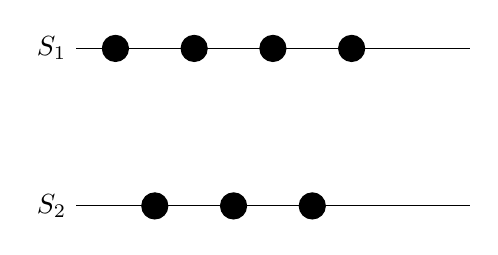
\begin{tikzpicture}

\draw (0, 0) node[left] {$S_2$} -- (5, 0);
\draw (0, 2) node[left] {$S_1$} -- (5, 2);

\tikzstyle{every node}+=[circle,draw,fill]

\node[circle,draw] (o1) at (1, 0) {};
\node[right of=o1] (o2) {};
\node[right of=o2] (o3) {};

\node (u1) at (0.5, 2) {};
\node[right of=u1] (u2) {};
\node[right of=u2] (u3) {};
\node[right of=u3] (u4) {};

\drawedges[bend right]{o1/o2,o1/o3,o2/o3}
\drawedges{o1/u1,o1/u2,o2/u2,o2/u3,o2/u4}
\drawedges[bend left]{u1/u4,u2/u3}

\end{tikzpicture}

Without caps: Level planarity solvable in linear time.\\{} 
[Jünger et al., 1999]
\end{frame}

\begin{frame}{Level planarity}
Level planarity is an ordering problem:
\begin{figure}[\placement]
\centering

%\resizebox{\textwidth}{!}{
\begin{tikzpicture}

%\tikzstyle{every node}+=[circle,draw]

\node (A1) {$a_1$};
\node[right of=A1] (A2) {$a_2$};
\node[below of=A1] (B2) {$b_2$};
\node[right of=B2] (B1) {$b_1$};
\draw (A1) edge (B1);
\draw (A2) edge (B2);

\begin{scope}[xshift=4cm]
\node (A1) {$a_1$};
\node[right of=A1] (A2) {$a_2$};
\node[below of=A1] (B1) {$b_1$};
\node[right of=B1] (B2) {$b_2$};
\draw (A1) edge (B1);
\draw (A2) edge (B2);
\end{scope}

\end{tikzpicture}
%}
\end{figure}
Forbidden: $a_1 <_i a_2 \land b_2 < b_1$ for $(a_1, b_1), (a_2, b_2) \in E_i$ 
\end{frame}

%\begin{frame}{Observations}
%
%Embeddability only depends on the order of the vertices on the spines:
%\begin{itemize}
%\item Caps come from page embedding
%\item Two edges between TODO
%\end{itemize}
%\end{frame}

\begin{frame}{Mapping to 2-page \probPTree}

\begin{theorem}
A \probMul instance is equivalent to a special 2-page \probPTree instance.
\end{theorem}

\begin{figure}[\placement]
\centering

\resizebox{0.90\textwidth}{!}{
\begin{tikzpicture}

%\draw (0, 0) node[left] {} -- (5, 0);
%\draw (0, -2) node[left] {} -- (5, -2);

%\tikzstyle{every node}+=[circle,draw,fill]

\node (a1) at (1, 0) {$a_1$};
\node[right of=a1] (a2) {$a_2$};
\node[right of=a2] (a3) {$a_3$};

\node (b1) at (0.5, -2) {$b_1$};
\node[right of=b1] (b2) {$b_2$};
\node[right of=b2] (b3) {$b_3$};
\node[right of=b3] (b4) {$b_4$};

\node (c1) at (0.5, -4) {$c_1$};
\node[right of=c1] (c2) {$c_2$};
\node[right of=c2] (c3) {$c_3$};
\node[right of=c3] (c4) {$c_4$};


\drawedges[bend left,edge2]{a1/a2,a1/a3,a2/a3}
\drawedges[edge1]{a1/b1,a1/b2,a2/b2,a2/b3,a2/b4}
\drawedges[edge2]{c1/b1,c1/b2,c2/b3,c2/b4}
\drawedges[bend right,edge1]{c1/c4,c1/c3}

\node[draw=none,fill=none] at (5.5,-2) {{\Huge $\rightsquigarrow$}};

\begin{scope}[xshift=7cm,yshift=-2cm]

%\draw (-1, 0) -- (9, 0);

\node (a1) at (0, 0) {$a_1$};
\node[right of=a1] (a2) {$a_2$};
\node[right of=a2] (a3) {$a_3$};

\node[right of=a3] (b4) {$b_4$};
\node[right of=b4] (b3) {$b_3$};
\node[right of=b3] (b2) {$b_2$};
\node[right of=b2] (b1) {$b_1$};

\node[right of=b1] (c1) {$c_1$};
\node[right of=c1] (c2) {$c_2$};
\node[right of=c2] (c3) {$c_3$};
\node[right of=c3] (c4) {$c_4$};

\drawedges[bend left,edge2]{a1/a2,a1/a3,a2/a3}
\drawedges[bend right,edge1]{a1/b1,a1/b2,a2/b2,a2/b3,a2/b4}
\drawedges[bend right,edge2]{c1/b1,c1/b2,c2/b3,c2/b4}
\drawedges[bend right,edge1]{c1/c4,c1/c3}

\end{scope}

\visible<2->{
\node[circle, draw] (r1) at ($ (a2) + (0, 4em) $) {};
\node[circle, draw] (r2) at ($ 0.5*($ (b2) + (b3) $) + (0, 4em)$) {};
\node[circle, draw] (r3) at ($ 0.5*($ (c2) + (c3) $) + (0, 4em)$) {};
\node[circle, draw] (r) at ($ (r2) + (0, 4em) $) {};
\drawedges[ultra thick]{r1/a1,r1/a2,r1/a3,r2/b1,r2/b2,r2/b3,r2/b4,r3/c1,r3/c2,r3/c3,r3/c4,r/r1,r/r2,r/r3}
}

\end{tikzpicture}
}
\end{figure}

\end{frame}